\documentclass{standalone}
\usepackage{pgfplots}
\pgfplotsset{compat=1.18}

\begin{document}

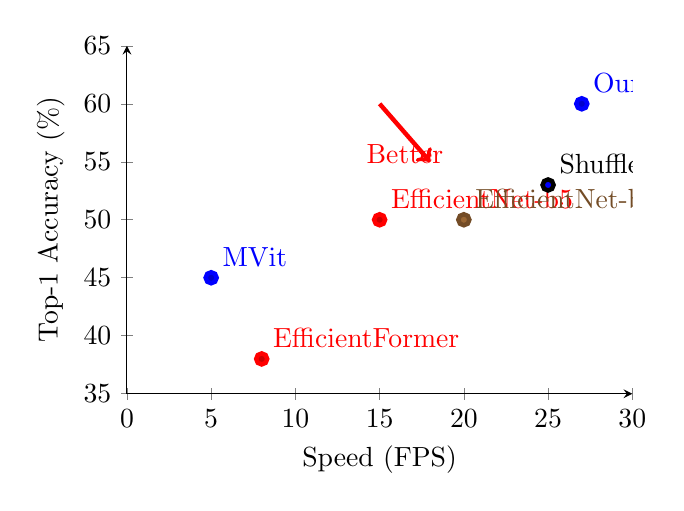
\begin{tikzpicture}
    \begin{axis}[
        width=8cm,
        height=6cm,
        xlabel={Speed (FPS)},
        ylabel={Top-1 Accuracy (\%)},
        xmin=0, xmax=30,
        ymin=35, ymax=65,
        xtick={0,5,...,29},
        ytick={35,40,...,65},
        axis lines=left,
        grid=none,
        every axis plot/.append style={ultra thick, mark options={solid}},
        ]
        % MVit
        \addplot+[only marks, fill=red, mark=*] coordinates {(5,45)} node[anchor=south west] {MVit};
        % EfficientNet-b5
        \addplot+[only marks, fill=yellow, mark=*] coordinates {(15,50)} node[anchor=south west] {EfficientNet-b5};
        % EfficientNet-b0
        \addplot+[only marks, fill=gray!50, mark=*] coordinates {(20,50)} node[anchor=south west] {EfficientNet-b0};
        % ShuffleNetV2
        \addplot+[only marks, fill=blue, mark=*] coordinates {(25,53)} node[anchor=south west] {ShuffleNetV2};
        % Ours
        \addplot+[only marks, fill=blue, mark=*] coordinates {(27,60)} node[anchor=south west] {Ours};
        % EfficientFormer
        \addplot+[only marks, fill=olive, mark=*] coordinates {(8,38)} node[anchor=south west] {EfficientFormer};
        
        % Red arrow indicating better performance
        \draw [->, ultra thick, red] (15, 60) -- (18, 55) node[midway, anchor=north] {Better};
    \end{axis}
\end{tikzpicture}

\caption{Top-1 accuracy, inference speed, and model size on the test set. The size of the circle denotes the model size, with smaller circles indicating fewer model parameters. The model closest to the top-right corner has the highest accuracy and the fastest inference. As indicated by the red arrow, performance is generally better towards this direction.}
\label{fig:performance_plot}
\end{document}